\documentclass[11pt,a4paper]{article}

\usepackage[utf8]{inputenc}
\usepackage[T1]{fontenc}
\usepackage[italian]{babel}
\usepackage{lmodern}
\usepackage{microtype}
\usepackage{geometry}
\geometry{margin=2.7cm}
\usepackage{amsmath,amssymb,amsthm,mathtools}
\usepackage{booktabs}
\usepackage{graphicx}
\usepackage{array}
\usepackage{enumitem}
\usepackage{xcolor}
\usepackage{hyperref}
\hypersetup{
  colorlinks=true,
  linkcolor=black,
  citecolor=black,
  urlcolor=blue,
  pdftitle={Un ordinamento strutturale ricorsivo delle parole basato su pivot vocalici},
  pdfauthor={Luca Montanelli}
}

\newtheorem{teorema}{Teorema}
\newtheorem{proposizione}[teorema]{Proposizione}
\newtheorem{lemma}[teorema]{Lemma}
\newtheorem{corollario}[teorema]{Corollario}
\theoremstyle{definition}
\newtheorem{definizione}[teorema]{Definizione}
\newtheorem{esempio}[teorema]{Esempio}
\theoremstyle{remark}
\newtheorem{osservazione}[teorema]{Osservazione}

\newcommand{\ARCA}{\mathrm{ARCA}}
\newcommand{\precA}{\prec_{\ARCA}}
\newcommand{\lexord}{\prec_{\mathrm{lex}}}
\newcommand{\Nrm}{N}
\newcommand{\Sig}{R}
\newcommand{\localSig}{\rho}
\newcommand{\Pivot}{p_w}
\newcommand{\Gap}{g_w}
\newcommand{\Vag}{W_w}
\newcommand{\Tag}{\tau_w}
\newcommand{\Class}{\eta}

\title{\textbf{Un ordinamento strutturale ricorsivo delle parole\\basato su pivot vocalici}\\[0.5em]
\large Formalizzazione matematica del metodo ARCA}
\author{Luca Montanelli}
\date{13/10/2026}

\begin{document}
\maketitle

\begin{abstract}
Si introduce un ordinamento delle parole alternativo all'ordinamento alfabetico diretto e inverso, sviluppato nell'ambito del progetto ARCA -- \emph{Assonanze, Rime, Consonanze e Anagrammi}. Il metodo associa a ogni parola una struttura ricorsiva ottenuta procedendo da destra verso sinistra attraverso particolari vocali di riferimento, dette \emph{pivot}. Due pivot consecutivi delimitano segmenti sovrapposti della parola, detti \emph{vagoni}. L'ordinamento non attribuisce uniformemente priorità alle lettere in base alla loro distanza dall'estremità della parola: la precedenza è determinata gerarchicamente dalla vocale finale corrente, dall'esistenza e dal valore del pivot, dalla distanza tra pivot e vocale finale e dalle lettere interne del vagone lette da destra verso sinistra. Iterando la costruzione, una parola viene trasformata in una rappresentazione strutturale ricorsiva finita. Si dimostra che, completata da criteri deterministici di disambiguazione, tale rappresentazione induce un ordine totale stretto sulle parole. Si studiano inoltre terminazione, complessità computazionale e contiguità delle classi definite da prefissi della firma. Un censimento empirico sull'intero vocabolario ARCA di 558.124 grafie misura il profilo probabilistico dei confronti e mostra che le parole adiacenti nell'ordine condividono prefissi strutturali molto più lunghi delle coppie uniformi, mentre le classi corrispondenti ai primi discriminanti della firma risultano effettivamente contigue.
\end{abstract}

\section{Introduzione}

Un ordinamento alfabetico tradizionale considera prioritariamente l'inizio della parola. Un dizionario inverso procede invece dalla fine verso l'inizio, confrontando i grafemi in ordine retrogrado. In entrambi i casi la parola viene trattata, ai fini dell'ordinamento, come una successione lineare uniforme di simboli.

Il metodo ARCA parte da un'idea differente: non tutte le posizioni della parola devono avere la stessa priorità strutturale. Le vocali vengono usate come punti di riferimento attraverso i quali la parola viene analizzata ricorsivamente in segmenti sovrapposti. Il confronto non procede quindi semplicemente carattere per carattere, ma attraverso una gerarchia di proprietà dei segmenti individuati.

La costruzione nasce dall'esigenza di organizzare un vocabolario in modo utile alla ricerca di rime, assonanze, consonanze e altre corrispondenze formali, senza richiedere, nella sua formulazione di base, una trascrizione fonetica completa.

\section{Contesto e relazione con approcci preesistenti}

Rimari e dizionari inversi sono strumenti lessicografici consolidati. Nei rimari le parole sono tipicamente raggruppate a partire dalla vocale tonica e dai suoni che la seguono; nei dizionari inversi i lemmi sono invece ordinati a partire dall'ultimo grafema e procedendo a ritroso \cite{crifo2011}. Sono stati inoltre proposti sistemi computazionali che modificano l'ordinamento retrogrado facendo intervenire informazione fonetica, vocali, consonanti e accento \cite{byrdchodorow1985}. In fonologia esistono anche rappresentazioni astratte che separano o schematizzano posizioni vocaliche e consonantiche, come i cosiddetti CV-skeleton \cite{boudelaa2004}. La ricerca di anteriorità svolta per questo lavoro ha considerato anche letteratura brevettuale relativa a rimari elettronici, ordinamenti fonetici e funzioni di \emph{sound-alike}; un esempio è il sistema MasterWriter, che ordina e filtra gruppi di rime sulla base di sillabe e informazione fonetica \cite{masterwriter2005}.

Il metodo qui formalizzato non coincide con tali costruzioni. La sua caratteristica specifica è la decomposizione ricorsiva basata sulla ricerca della prima vocale non adiacente alla vocale finale corrente, sulla promozione di tale vocale a \emph{pivot}, sulla definizione di segmenti sovrapposti (i \emph{vagoni}) e sull'iterazione della stessa regola prendendo il pivot appena trovato come nuova vocale finale.

\medskip
\noindent\textbf{Dichiarazione di originalità.} Il metodo di ordinamento strutturale di ARCA è un metodo originale sviluppato da \textbf{Luca Montanelli}. Per quanto emerso dalla ricerca bibliografica e tecnica svolta per questo lavoro, non è stata individuata in letteratura una costruzione antecedente equivalente basata sulla decomposizione ricorsiva in vagoni e pivot qui definita. Questa affermazione descrive lo stato della ricerca svolta e non costituisce una certificazione assoluta di prior art o di novità brevettuale.

\section{Impostazione formale}

Sia $\Sigma$ un alfabeto finito dotato di un ordine totale $<_{\Sigma}$. Una parola è una stringa finita
\[
  w=x_0x_1\dots x_{n-1},\qquad x_i\in\Sigma.
\]
Gli indici partono da $0$.

Sia $V\subseteq\Sigma$ l'insieme dei simboli considerati vocali. Nell'istanza italiana di base,
\[
  V=\{a,e,i,o,u\}.
\]

Per separare la teoria astratta dai dettagli di codifica, introduciamo una funzione deterministica di normalizzazione
\[
  \Nrm:\Sigma^*\longrightarrow\Sigma^*.
\]
Nell'implementazione corrente di ARCA, la chiave di rimario converte le lettere ASCII maiuscole in minuscole e riconduce le vocali italiane con accento grave o acuto alla corrispondente vocale base ai soli fini dell'ordinamento. La grafia originale viene comunque conservata per l'eventuale disambiguazione finale.

Da questo punto in avanti, salvo diversa indicazione, la parola considerata è la parola normalizzata $\Nrm(w)$.

\section{Vocale finale, pivot e vagone}

\begin{definizione}[Vocale finale strutturale]
Se $w$ contiene almeno una vocale, definiamo la posizione della sua vocale finale strutturale come
\[
  f(w)=\max\{i\in\{0,\dots,n-1\}:x_i\in V\}.
\]
Il simbolo $x_{f(w)}$ è detto \emph{vocale finale corrente}.
\end{definizione}

La vocale finale strutturale non deve necessariamente coincidere con l'ultimo carattere della parola: eventuali consonanti poste dopo l'ultima vocale non fanno parte della decomposizione principale e intervengono soltanto nei criteri finali di disambiguazione.

\begin{definizione}[Pivot]
Sia $f$ la posizione della vocale finale corrente. Il pivot associato a $f$ è
\[
  \Pivot(f)=\max\{i\leq f-2:x_i\in V\},
\]
quando tale insieme non è vuoto. Se l'insieme è vuoto, diciamo che il pivot non esiste.
\end{definizione}

La condizione $i\leq f-2$ formalizza il requisito di \emph{non adiacenza}: una vocale in posizione $f-1$ è immediatamente adiacente alla vocale corrente e non può fungere da pivot.

\begin{definizione}[Vagone e gap]
Se il pivot $p=\Pivot(f)$ esiste, definiamo il vagone
\[
  \Vag(p,f)=x_px_{p+1}\dots x_f.
\]
Il numero di caratteri strettamente compresi tra pivot e vocale finale è il \emph{gap}
\[
  \Gap(p,f)=f-p-1.
\]
La lunghezza del vagone è quindi $\Gap(p,f)+2$.
\end{definizione}

Definiamo inoltre l'interno del vagone letto da destra verso sinistra:
\[
  I_w(p,f)=(x_{f-1},x_{f-2},\dots,x_{p+1}).
\]
La lunghezza di $I_w(p,f)$ è esattamente $\Gap(p,f)$.

\section{Catena ricorsiva dei pivot}

Poniamo
\[
  f_0=f(w).
\]
Se $\Pivot(f_0)$ esiste, definiamo
\[
  f_1=\Pivot(f_0).
\]
Ricorsivamente, finché il pivot esiste,
\[
  f_{k+1}=\Pivot(f_k).
\]
Si ottiene una successione
\[
  f_0>f_1>\dots>f_r.
\]

I vagoni consecutivi non formano una partizione disgiunta della parola. Il pivot di un vagone diventa infatti la vocale finale del vagone successivo: la stessa posizione appartiene quindi a due livelli consecutivi della costruzione. È più corretto pensare alla decomposizione come a una catena di finestre sovrapposte.

\begin{proposizione}[Terminazione e numero massimo di livelli]
Per ogni parola finita $w=x_0\dots x_{n-1}$, con $n\geq 1$, contenente almeno una vocale, la costruzione ricorsiva dei pivot termina dopo un numero finito di passi. Se
\[
  f_0=f(w)
\]
è la posizione della vocale finale strutturale e la catena contiene $L(w)$ livelli, allora
\[
  L(w)\leq \left\lfloor\frac{f_0}{2}\right\rfloor+1
  \leq \left\lceil\frac{n}{2}\right\rceil.
\]
Entrambi i limiti sono raggiungibili.
\end{proposizione}

\begin{proof}
Per definizione di pivot, a ogni livello successivo la nuova vocale finale si trova almeno due posizioni a sinistra della precedente:
\[
  f_{j+1}\leq f_j-2.
\]
Iterando,
\[
  f_j\leq f_0-2j.
\]
Un livello di indice $j$ può esistere soltanto se $f_j\geq0$; pertanto
\[
  f_0-2j\geq0,
  \qquad
  j\leq\left\lfloor\frac{f_0}{2}\right\rfloor.
\]
Se i livelli sono indicizzati da $0$ a $r$, il loro numero è $L(w)=r+1$, da cui
\[
  L(w)\leq\left\lfloor\frac{f_0}{2}\right\rfloor+1.
\]
Poiché $f_0\leq n-1$,
\[
  L(w)\leq\left\lfloor\frac{n-1}{2}\right\rfloor+1
  =\left\lceil\frac{n}{2}\right\rceil.
\]
Il limite è netto: per $n$ pari si possono collocare le vocali strutturali nelle posizioni
$n-1,n-3,\dots,1$, mentre per $n$ dispari nelle posizioni
$n-1,n-3,\dots,0$. In entrambi i casi ogni nuova vocale ammissibile diventa il pivot del livello precedente e si ottiene esattamente $\lceil n/2\rceil$ livelli.
\end{proof}

\begin{osservazione}
Per esempio, se $n=8$ gli indici disponibili sono $0,\dots,7$ e una catena massimale può avere posizioni $7,5,3,1$: i livelli sono quindi $4=\lceil8/2\rceil$. Se $n=9$, le posizioni $8,6,4,2,0$ realizzano invece $5=\lceil9/2\rceil$ livelli. La formulazione tramite $f_0$ separa il numero di caratteri dall'indice dell'ultima vocale ed evita l'ambiguità dovuta all'indicizzazione a partire da zero.
\end{osservazione}

\section{Regola locale di confronto}

Consideriamo due parole al medesimo livello ricorsivo e supponiamo che le loro vocali finali correnti siano nelle posizioni $f_u$ e $f_v$.

Il confronto segue questa gerarchia:
\begin{enumerate}[label=\arabic*.]
  \item vocale finale corrente;
  \item esistenza o assenza del pivot;
  \item valore della vocale pivot, se il pivot esiste in entrambe;
  \item gap, cioè numero di caratteri tra pivot e vocale finale;
  \item lettere interne del vagone, lette da destra verso sinistra;
  \item se tutti i dati precedenti coincidono, prosecuzione ricorsiva usando il pivot come nuova vocale finale.
\end{enumerate}

Se una parola non possiede pivot al livello corrente e l'altra sì, la parola senza pivot precede quella con pivot. Questa scelta è parte della definizione dell'ordinamento.

\section{Il caso terminale}

Quando il pivot non esiste, la ricorsione termina. Se $f$ è la posizione della vocale finale corrente, il segmento residuo è
\[
  T(w,f)=x_0x_1\dots x_f.
\]
Il confronto terminale avviene nel seguente ordine:
\begin{enumerate}[label=\arabic*.]
  \item posizione $f$ della vocale finale, equivalente al numero di caratteri che la precedono;
  \item a parità di $f$, caratteri $x_{f-1},x_{f-2},\dots,x_0$ in quest'ordine, cioè procedendo da destra verso sinistra.
\end{enumerate}

Si osservi che questa regola non attribuisce priorità alla parte sinistra della parola prima dei vagoni più a destra. Al contrario, la parte sinistra viene esaminata soltanto dopo che tutti i livelli strutturali precedenti sono risultati uguali.

\section{Esempi elementari}

\begin{esempio}[$\texttt{afa}$ e $\texttt{ala}$]
Entrambe le parole hanno vocale finale $a$, pivot $a$ e gap $1$. La prima differenza è quindi nella lettera interna:
\[
  f<_{\Sigma}l.
\]
Pertanto
\[
  \texttt{afa}\precA\texttt{ala}.
\]
\end{esempio}

\begin{esempio}[$\texttt{afa}$ e $\texttt{acca}$]
Le due parole hanno la stessa vocale finale e lo stesso pivot. Tuttavia
\[
  g_{\texttt{afa}}=1,\qquad g_{\texttt{acca}}=2.
\]
Il gap ha priorità sulle lettere interne, quindi
\[
  \texttt{afa}\precA\texttt{acca}
\]
senza necessità di confrontare $f$ con $c$.
\end{esempio}

\section{Esempio ricorsivo: \texttt{caramella} e \texttt{gargamella}}

Consideriamo
\[
  w=\texttt{caramella}.
\]
La parola contiene nove lettere, indicizzate da $0$ a $8$:
\[
\begin{array}{c|ccccccccc}
 i   &0&1&2&3&4&5&6&7&8\\
\hline
 x_i &c&a&r&a&m&e&l&l&a
\end{array}
\]
La vocale finale è quindi la $a$ in posizione $8$. Il primo pivot è la $e$ in posizione $5$, e il primo vagone è
\[
  \boxed{\texttt{ella}}.
\]
La $e$ in posizione $5$ diventa ora la nuova vocale finale. Il pivot successivo è la $a$ in posizione $3$, da cui
\[
  \boxed{\texttt{ame}}.
\]
La $a$ in posizione $3$ diventa la nuova vocale finale; il pivot successivo è la $a$ in posizione $1$, da cui
\[
  \boxed{\texttt{ara}}.
\]
Infine, rispetto alla $a$ in posizione $1$, non esiste alcun pivot. Il segmento terminale è
\[
  \boxed{\texttt{ca}}.
\]
Possiamo quindi visualizzare informalmente la struttura come
\[
  \texttt{caramella}\longmapsto
  [\texttt{ella},\texttt{ame},\texttt{ara},\texttt{ca}].
\]
Questa notazione è soltanto illustrativa: non rappresenta una partizione, poiché vagoni consecutivi condividono la vocale pivot.

Per
\[
  \texttt{gargamella}
\]
si ottiene analogamente
\[
  [\texttt{ella},\texttt{ame},\texttt{arga},\texttt{ga}].
\]
I primi due livelli coincidono. La prima differenza compare tra $\texttt{ara}$ e $\texttt{arga}$. Le vocali estreme coincidono, ma i gap sono rispettivamente $1$ e $2$; pertanto
\[
  \texttt{caramella}\precA\texttt{gargamella}.
\]

\section{Firma strutturale ricorsiva}

Per formalizzare l'intera costruzione introduciamo due tipi di record ricorsivi: un record \emph{terminale} e un record \emph{ricorsivo}.

\begin{definizione}[Indicatore di pivot]
Per una parola $w$ e una vocale finale corrente in posizione $f$, poniamo
\[
  \Tag(f)=
  \begin{cases}
    0, & \text{se }\Pivot(f)\text{ non esiste},\\
    1, & \text{se }\Pivot(f)\text{ esiste}.
  \end{cases}
\]
\end{definizione}

La scelta numerica $0<1$ non è arbitraria: traduce direttamente la regola secondo cui, a parità di vocale finale, un livello senza pivot deve precedere un livello con pivot. Il bit $\Tag(f)$ è quindi un \emph{discriminante di tipo}: permette di confrontare in modo uniforme i due possibili casi della definizione ricorsiva.

\begin{definizione}[Firma locale]
Se il pivot non esiste, definiamo
\[
  \localSig(w,f)=
  \Bigl(
    x_f,\,0,\,f,\,x_{f-1},x_{f-2},\dots,x_0
  \Bigr).
\]
Se invece $p=\Pivot(f)$ esiste, definiamo
\[
  \localSig(w,f)=
  \Bigl(
    x_f,\,1,\,x_p,\,f-p-1,\,
    x_{f-1},\dots,x_{p+1},\,
    \localSig(w,p)
  \Bigr).
\]
Il confronto tra firme locali segue esattamente l'ordine dei campi appena scritto.
\end{definizione}

\begin{definizione}[Firma strutturale ARCA]
Per una parola normalizzata contenente almeno una vocale, definiamo
\[
  \Sig(w)=\localSig(w,f(w)).
\]
\end{definizione}

La firma $\Sig(w)$ non è una semplice stringa rovesciata: è un oggetto ricorsivo la cui forma dipende dalla posizione delle vocali nella parola.

\section{La chiave completa e il significato del marcatore $0/1$}

La firma $\Sig(w)$ è definita soltanto per parole contenenti almeno una vocale. Occorre quindi un secondo indicatore, distinto da $\Tag(f)$, per collocare nello stesso ordinamento anche le parole prive di vocali.

\begin{definizione}[Indicatore di classe della parola]
Poniamo
\[
  \Class(w)=
  \begin{cases}
    0, & \text{se }\Nrm(w)\text{ contiene almeno una vocale},\\
    1, & \text{se }\Nrm(w)\text{ non contiene vocali}.
  \end{cases}
\]
\end{definizione}

Anche qui la scelta $0<1$ codifica una decisione dell'ordinamento: le parole dotate di struttura vocalica devono precedere le parole prive di vocali.

È importante non confondere i due indicatori:
\begin{itemize}
  \item $\Tag(f)$ è \emph{locale}: dice se, al livello ricorsivo corrente, esiste un pivot;
  \item $\Class(w)$ è \emph{globale}: dice se la parola possiede almeno una vocale e quindi ammette una firma strutturale ARCA.
\end{itemize}

Definiamo la chiave completa
\[
  K(w)=
  \begin{cases}
    \bigl(0,\Sig(\Nrm(w)),\Nrm(w),w\bigr),
      & \text{se }\Class(w)=0,\\[0.4em]
    \bigl(1,\Nrm(w),w\bigr),
      & \text{se }\Class(w)=1.
  \end{cases}
\]

I campi $\Nrm(w)$ e $w$ alla fine della chiave sono \emph{tie-breaker}: intervengono soltanto quando la struttura rimaria non ha distinto le due parole. Sono necessari perché la normalizzazione può far coincidere grafie originariamente diverse, per esempio nel trattamento di maiuscole e vocali accentate.

L'ordinamento ARCA è definito da
\[
  u\precA v
  \quad\Longleftrightarrow\quad
  K(u)\lexord K(v),
\]
dove il confronto è lessicografico secondo gli ordini totali fissati sui singoli campi e secondo il confronto ricorsivo delle firme.

\section{L'ordinamento è totale}

Per evitare ambiguità, dimostriamo prima che il confronto tra firme ricorsive è ben definito e totale.

\begin{lemma}[Ordine totale sulle firme]
Il confronto ricorsivo tra firme strutturali ARCA definito sopra è un ordine totale stretto sull'insieme delle firme finite.
\end{lemma}

\begin{proof}
Procediamo per induzione sulla profondità massima delle due firme considerate.

\emph{Caso base.} Se entrambe le firme sono terminali, esse hanno la forma
\[
  (x_f,0,f,x_{f-1},\dots,x_0).
\]
I campi vengono confrontati lessicograficamente. L'ordine su $\Sigma$ è totale, l'ordine sugli interi non negativi è totale e l'ordine lessicografico su sequenze finite di elementi totalmente ordinati è totale. Quindi due firme terminali sono sempre confrontabili; il confronto è irriflessivo e transitivo.

\emph{Passo induttivo.} Supponiamo che il risultato valga per tutte le firme di profondità al più $d$. Consideriamo due firme di profondità al più $d+1$.

Prima si confronta la vocale finale. Se differisce, il confronto è deciso dall'ordine totale su $\Sigma$. Se coincide, si confronta il marcatore locale $\Tag\in\{0,1\}$. Se i marcatori differiscono, il confronto è deciso da $0<1$.

Se entrambi i marcatori sono $0$, siamo nel caso terminale già trattato. Se entrambi sono $1$, si confrontano nell'ordine la vocale pivot, il gap e la sequenza interna del vagone. Tutti questi campi appartengono a insiemi totalmente ordinati. Soltanto se essi coincidono si arriva al confronto delle firme figlie $\localSig(w,p)$, che hanno profondità al più $d$ e sono quindi totalmente ordinate per ipotesi induttiva.

In ogni caso il confronto si riduce, dopo un numero finito di passi, al confronto di elementi appartenenti a insiemi totalmente ordinati. La costruzione è lessicografica e preserva irriflessività, transitività e tricotomia. Ne segue che il confronto sulle firme è un ordine totale stretto.
\end{proof}

\begin{teorema}[Ordine totale stretto sulle parole]
Fissati l'alfabeto ordinato $\Sigma$, l'insieme vocalico $V$ e la normalizzazione deterministica $\Nrm$, la relazione $\precA$ definisce un ordine totale stretto sull'insieme delle parole distinte considerate dal sistema.
\end{teorema}

\begin{proof}
Per la Proposizione 1, la firma $\Sig(\Nrm(w))$ di ogni parola contenente vocali è finita. Per il Lemma precedente, l'insieme delle firme finite è dotato di un ordine totale stretto.

Consideriamo ora due parole distinte $u$ e $v$.

Se $\Class(u)\neq\Class(v)$, il primo campo delle chiavi è rispettivamente $0$ e $1$, quindi esattamente una delle due relazioni $K(u)\lexord K(v)$ o $K(v)\lexord K(u)$ è vera.

Se entrambe le parole appartengono alla classe vocalica, si confrontano prima le firme $\Sig(\Nrm(u))$ e $\Sig(\Nrm(v))$. Se esse differiscono, il Lemma decide univocamente l'ordine. Se coincidono, si confrontano $\Nrm(u)$ e $\Nrm(v)$ con l'ordine lessicografico su stringhe. Se anche le normalizzazioni coincidono, si confrontano infine le grafie originali $u$ e $v$. Poiché $u\neq v$, quest'ultimo confronto risolve necessariamente il pareggio.

Se entrambe le parole sono prive di vocali, il confronto avviene direttamente su $\Nrm(u)$ e $\Nrm(v)$ e, in caso di ulteriore uguaglianza, sulle grafie originali.

Ne segue la tricotomia: per $u\neq v$ vale esattamente una tra
\[
  u\precA v
  \qquad\text{e}\qquad
  v\precA u.
\]
L'irriflessività segue dal fatto che nessuna chiave è lessicograficamente minore di sé stessa. La transitività segue dalla transitività degli ordini lessicografici usati in ciascun campo e, per le firme, dal Lemma precedente. Pertanto $\precA$ è un ordine totale stretto.
\end{proof}

\section{Parole prive di vocali e suffissi consonantici}

Le parole prive di vocali non ammettono la decomposizione in pivot e vagoni. Per definizione, esse appartengono alla classe $\Class=1$ e vengono quindi dopo tutte le parole della classe vocalica. Tra loro si usa la chiave normalizzata e, in caso di ulteriore parità, la grafia originale.

Le consonanti poste dopo l'ultima vocale di una parola non modificano la firma strutturale principale, poiché la costruzione parte dalla posizione $f(w)$ dell'ultima vocale. Tali caratteri rimangono tuttavia presenti in $\Nrm(w)$ e possono quindi distinguere due parole la cui firma strutturale sia identica.

\section{Differenza rispetto a un ordinamento inverso}

In un dizionario inverso la priorità è determinata esclusivamente dalla distanza dei grafemi dalla fine della parola:
\[
  x_{n-1},x_{n-2},x_{n-3},\dots.
\]
Nel metodo ARCA, invece, la successione delle priorità dipende dalla struttura vocalica della parola. Un'informazione relativa a un pivot o al gap può avere priorità rispetto a caratteri geometricamente più vicini alla fine. Due caratteri collocati a distanze differenti dall'estremità possono inoltre essere confrontati allo stesso livello ricorsivo se svolgono lo stesso ruolo strutturale.

Questa è la differenza essenziale tra un ordinamento retrogrado lineare e un ordinamento strutturale ricorsivo.

\section{Complessità computazionale}

In questa sezione distinguiamo problemi diversi: costruire la firma, confrontare due parole, ordinare un vocabolario e cercare una classe strutturale all'interno di un vocabolario già ordinato. A questi aspetti teorici affianchiamo una verifica empirica sull'intero vocabolario ARCA corrente. È importante non confondere il costo di costruzione della rappresentazione con il costo di un confronto, né il costo di un singolo confronto con quello di una query su un indice già costruito.

Siano $\ell_u=|\Nrm(u)|$ e $\ell_v=|\Nrm(v)|$ le lunghezze delle due parole considerate, e sia $L=\max(\ell_u,\ell_v)$.

\subsection{Costruzione della firma}

La posizione dell'ultima vocale e tutti i pivot successivi possono essere determinati con una singola scansione da destra verso sinistra. Una volta incontrato un pivot, la scansione prosegue soltanto nella parte ancora non esaminata. Ogni posizione della parola viene quindi visitata un numero limitato di volte.

\begin{proposizione}[Costo di costruzione]
La firma strutturale di una parola di lunghezza $\ell$ può essere costruita in tempo $\Theta(\ell)$ e occupa spazio $\Theta(\ell)$ se viene materializzata integralmente.
\end{proposizione}

\begin{proof}
Ogni carattere deve essere letto almeno una volta nel caso peggiore, quindi il costo è $\Omega(\ell)$. Una scansione monotona da destra verso sinistra è sufficiente per individuare ultima vocale, pivot, gap e interni dei vagoni, senza tornare su intervalli già elaborati se non per un numero costante di estremi condivisi. Il costo è quindi anche $O(\ell)$. La firma contiene complessivamente una quantità lineare di informazione rispetto alla parola, da cui lo stesso ordine di grandezza per lo spazio.
\end{proof}

\subsection{Confronto tra due firme precomputate}

Se le firme sono già disponibili, il confronto può terminare molto presto. Per esempio, se le vocali finali differiscono, basta il primo discriminante strutturale. Se le vocali finali coincidono ma differisce l'indicatore di pivot, basta il secondo discriminante. Lo stesso vale, in successione, per pivot, gap e lettere interne.

\begin{proposizione}[Caso migliore e caso peggiore]
Per firme precomputate, il confronto tra due parole ha costo
\[
  \Theta(1) \quad\text{nel caso migliore},
\]
\[
  \Theta(\ell_u+\ell_v) \quad\text{nel caso peggiore}.
\]
\end{proposizione}

\begin{proof}
Nel caso migliore il primo campo confrontato è già diverso, per esempio la vocale finale, e il confronto termina dopo un numero costante di operazioni. Nel caso peggiore le due strutture coincidono per quasi tutta la loro estensione, oppure sono identiche strutturalmente e occorre arrivare ai tie-breaker finali. Poiché ciascun simbolo dei vagoni attraversati viene esaminato al più un numero costante di volte, il numero totale di confronti elementari è lineare nella somma delle lunghezze.
\end{proof}

\subsection{Caso medio: profilo di sopravvivenza e probabilità condizionate}

Non esiste una complessità media unica senza specificare una distribuzione sulle parole e una convenzione precisa per ciò che viene contato. Fissiamo quindi una codifica sequenziale della firma coerente con la gerarchia del comparatore e indichiamo con $C(u,v)$ il numero di discriminanti elementari esaminati prima della decisione. Il valore numerico di $C$ dipende dalla codifica scelta: per esempio una codifica fedele all'implementazione può conservare confronti ridondanti che un encoder più compatto potrebbe evitare. Le identità probabilistiche seguenti, invece, valgono per qualunque scelta fissata di $C$.

Per $k\geq1$ definiamo la funzione di sopravvivenza
\[
  S_k=\Pr(C\geq k)
\]
e, quando $S_k>0$, la probabilità condizionata di prosecuzione
\[
  q_k=\Pr(C\geq k+1\mid C\geq k)
      =\frac{S_{k+1}}{S_k}.
\]
In parole, $S_k$ misura la probabilità che il confronto debba arrivare almeno al $k$-esimo discriminante; $q_k$ misura invece, sapendo che il confronto è già arrivato al $k$-esimo discriminante, la probabilità che anche questo non basti e sia necessario proseguire.

\begin{proposizione}[Identità del profilo $q_k$]
Se $C$ è una variabile aleatoria intera positiva e finita, allora
\[
  S_1=1,
  \qquad
  S_k=\prod_{j=1}^{k-1}q_j\quad(k\geq2),
\]
e
\[
  \mathbb{E}[C]
  =\sum_{k\geq1}S_k
  =1+q_1+q_1q_2+q_1q_2q_3+\cdots.
\]
\end{proposizione}

\begin{proof}
Dalla definizione di probabilità condizionata,
\[
  S_{k+1}=q_kS_k.
\]
Poiché $S_1=1$, iterando si ottiene
\[
  S_k=q_1q_2\cdots q_{k-1}.
\]
Per una variabile aleatoria intera positiva vale inoltre la formula delle code
\[
  \mathbb{E}[C]=\sum_{k\geq1}\Pr(C\geq k),
\]
che fornisce l'identità dichiarata.
\end{proof}

\begin{corollario}[Maggiorazione geometrica]
Se esiste una costante $q<1$ tale che
\[
  q_k\leq q
\]
per ogni $k$ per cui $q_k$ è definita, allora
\[
  \mathbb{E}[C]\leq\frac{1}{1-q}.
\]
\end{corollario}

\begin{proof}
Dalla proposizione precedente,
\[
  S_k=\prod_{j=1}^{k-1}q_j\leq q^{k-1}.
\]
Pertanto
\[
  \mathbb{E}[C]
  =\sum_{k\geq1}S_k
  \leq\sum_{k\geq1}q^{k-1}
  =\frac{1}{1-q}.
\]
\end{proof}

Il corollario conserva il modello geometrico semplice, ma non deve essere confuso con una legge empirica dell'ordinamento ARCA. I diversi discriminanti hanno significati differenti e le probabilità $q_k$ non sono in generale uguali. Inoltre, ai livelli ricorsivi successivi, la vocale finale corrente coincide con il pivot già confrontato al livello precedente: in una codifica fedele al comparatore quel particolare controllo può quindi avere probabilità condizionata pari a $1$. Per descrivere il comportamento reale risultano più informative la curva $S_k$, la sequenza completa dei $q_k$ e le probabilità associate ai singoli stadi strutturali.

\begin{osservazione}[Confronto con l'ordine alfabetico]
Anche il normale confronto lessicografico da sinistra verso destra ha caso migliore $\Theta(1)$, caso peggiore $\Theta(L)$ e, sotto opportune distribuzioni, può avere costo medio limitato. L'eventuale vantaggio algoritmico di ARCA non consiste quindi nel fatto che \emph{ogni confronto di due parole} sia asintoticamente più veloce di un confronto alfabetico. Il punto centrale è piuttosto che l'ordinamento ARCA rende contigue le classi definite da prefissi della propria firma strutturale.
\end{osservazione}

\subsection{Conteggio esatto dei profili sul vocabolario}

Le quantità $S_k$ e $q_k$ possono essere misurate sull'intero vocabolario senza enumerare esplicitamente tutte le coppie di parole. Siano $M$ le grafie del corpus e
\[
  T=\binom{M}{2}
\]
il numero delle coppie non ordinate. Per ogni $p\geq0$, raggruppiamo le parole che condividono i primi $p$ campi della firma. Se $\mathcal{G}_p$ è l'insieme di tali gruppi, poniamo
\[
  A_p=\sum_{G\in\mathcal{G}_p}\binom{|G|}{2}.
\]
Allora $A_p$ è esattamente il numero di coppie che coincidono nei primi $p$ discriminanti e
\[
  S_k=\frac{A_{k-1}}{T},
  \qquad
  q_k=\frac{A_k}{A_{k-1}}
\]
quando $A_{k-1}>0$. Questo rende possibile un censimento combinatorio esatto del profilo anche quando $T$ è dell'ordine di $10^{11}$.

\subsection{Verifica empirica sull'intero vocabolario ARCA}

È stato eseguito un benchmark riproducibile sullo snapshot del progetto ARCA identificato dal commit
\texttt{2d87314e12191fa5d0d4d3d26e40c9fcc0c81f22}. Il vocabolario contiene $558\,124$ grafie e ha SHA-256
\texttt{b3b5703f69874095e9f9ac630ed0a608b919d969d5cd3a6b6477735db8595ad6}. Il numero totale di coppie non ordinate è
\[
  \binom{558124}{2}=155\,750\,920\,626.
\]
Il benchmark è stato eseguito in C++17, a singolo thread, su Windows 11 con CPU AMD Ryzen 3 3250U e GCC 15.2.0. Le misure temporali dipendono da questa piattaforma; i conteggi combinatori e le proprietà di contiguità, invece, dipendono dallo snapshot del corpus e dall'ordinamento considerato.

La firma sperimentale è stata validata contro il comparatore di produzione su tutte le $558\,123$ coppie adiacenti, su due milioni di coppie non adiacenti deterministiche e mediante riordinamento completo delle $558\,124$ grafie. I conteggi del profilo sono stati inoltre verificati con due procedimenti combinatori indipendenti.

Nel modello sperimentale $C_{\mathrm{struct}}$ conta soltanto i campi della struttura ARCA, mentre $C_{\mathrm{total}}$ include anche i tie-breaker della chiave normalizzata e della grafia originale. Un'unità di costo è il confronto di un campo scalare omologo; non equivale a un'istruzione CPU, a una lettura di cache o a un tempo fisso.

\begin{table}[htbp]
\centering
\caption{Distribuzione empirica di $C_{\mathrm{total}}$ per differenti popolazioni di coppie.}
\label{tab:costo-empirico}
\resizebox{\textwidth}{!}{%
\begin{tabular}{lrrrrrrrrr}
\toprule
Distribuzione & Coppie/occorrenze & $\mathbb{E}[C]$ & Mediana & SD & P90 & P95 & P99 & P99.9 & Max \\
\midrule
Uniformi & 155750920626 & 2,830372 & 2 & 1,656115 & 4 & 6 & 10 & 16 & 76 \\
Adiacenti ARCA & 558123 & 19,138855 & 19 & 5,533859 & 26 & 28 & 35 & 49 & 76 \\
Stessa vocale finale & 45367372759 & 4,854282 & 4 & 1,905980 & 6 & 9 & 15 & 20 & 76 \\
Stessa finale e pivot & 15019564687 & 6,588921 & 6 & 2,542891 & 10 & 12 & 16 & 21 & 76 \\
\bottomrule
\end{tabular}%
}
\end{table}

Per le coppie uniformi si ottiene
\[
  \mathbb{E}[C_{\mathrm{total}}]\simeq2{,}830372,
\]
mentre per coppie adiacenti nell'ordine ARCA
\[
  \mathbb{E}[C_{\mathrm{total}}]\simeq19{,}138855.
\]
Il secondo valore è circa $6{,}76$ volte il primo. Questo non significa che l'ordinamento sia meno efficiente: le coppie adiacenti sono, per costruzione, fortemente selezionate e condividono prefissi strutturali molto più lunghi. Il dato fornisce invece evidenza empirica che l'ordinamento aggrega effettivamente parole che risultano simili secondo la struttura ARCA. La stessa progressione è visibile passando dalle coppie uniformi alle coppie condizionate ad avere la stessa vocale finale e poi la stessa coppia vocale finale--pivot.

La distinzione fra costo strutturale e costo completo è piccola nella media uniforme ma diventa più visibile fra le adiacenze:
\begin{table}[htbp]
\centering
\caption{Confronto tra costo strutturale e costo totale.}
\label{tab:struct-total}
\begin{tabular}{lrrrr}
\toprule
Distribuzione & $\mathbb{E}[C_{\mathrm{struct}}]$ & $\mathbb{E}[C_{\mathrm{total}}]$ & Mediana struct & Max struct \\
\midrule
Uniformi & 2,830370 & 2,830372 & 2 & 48 \\
Adiacenti ARCA & 18,819242 & 19,138855 & 18 & 48 \\
Stessa vocale finale & 4,854278 & 4,854282 & 4 & 48 \\
Stessa finale e pivot & 6,588909 & 6,588921 & 6 & 48 \\
\bottomrule
\end{tabular}
\end{table}

La differenza fra le varie distribuzioni è visualizzata anche dalla Figura~\ref{fig:profilo-q}. Le curve di sopravvivenza $S_k=P(C_{\mathrm{total}}\ge k)$ decadono molto rapidamente per le coppie uniformi, più lentamente per le coppie condizionate e molto più lentamente per le coppie adiacenti nell'ordine ARCA. Questo comportamento non è un accidente statistico: indica che parole vicine secondo ARCA condividono prefissi strutturali sensibilmente più lunghi di quanto accada per due parole scelte a caso nel vocabolario. In questo senso il benchmark fornisce evidenza empirica che l'ordinamento realizza il proprio obiettivo progettuale di aggregare parole strutturalmente simili secondo la logica ARCA.

\begin{figure}[htbp]
\centering
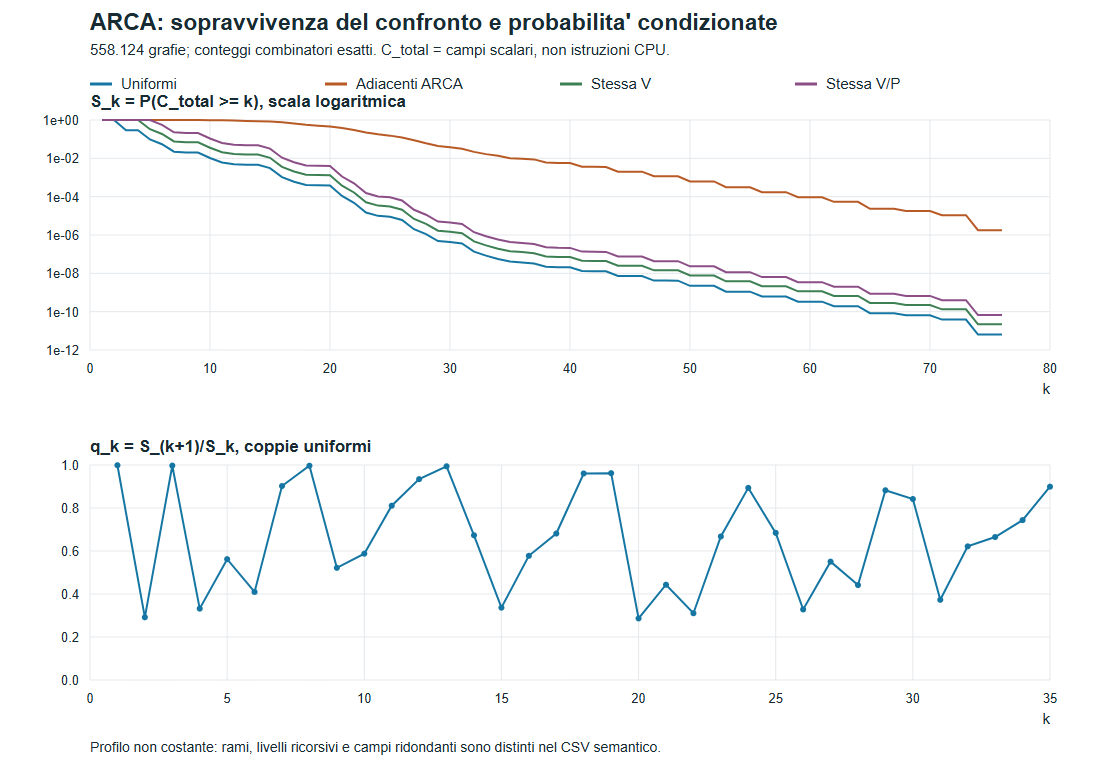
\includegraphics[width=0.96\textwidth]{profilo_q.png}
\caption{Profili empirici di sopravvivenza $S_k$ e probabilità condizionate $q_k$ sul vocabolario ARCA. La curva delle adiacenze ARCA decresce molto più lentamente di quella delle coppie uniformi, segnalando prefissi strutturali condivisi significativamente più lunghi.}
\label{fig:profilo-q}
\end{figure}

\subsection{Probabilità semanticamente interpretabili}

Il profilo posizionale $q_k$ può essere affiancato da probabilità condizionate associate ai diversi stadi della struttura. Al primo livello ricorsivo, sul corpus considerato, si osservano i valori della Tabella~\ref{tab:q-semantiche}.

\begin{table}[htbp]
\centering
\caption{Prime probabilità condizionate semanticamente interpretabili.}
\label{tab:q-semantiche}
\begin{tabular}{lrrr}
\toprule
Stadio & Coppie in ingresso & Coppie che proseguono & $q$ \\
\midrule
Vocale finale $V$ & 155590780366 & 45367372759 & 0,291581 \\
Stato pivot $\tau$ & 45367372759 & 45239410378 & 0,997179 \\
Vocale pivot $P$ & 45239286624 & 15019564687 & 0,332003 \\
Gap $G$ & 15019564687 & 8441938139 & 0,562063 \\
Prima lettera interna $I_1$ & 8441938139 & 3456604528 & 0,409456 \\
\bottomrule
\end{tabular}
\end{table}

Per esempio, $q_V\simeq0{,}2916$ significa che, tra le coppie che entrano nel primo livello vocalico, circa il $29{,}16\%$ condivide la vocale finale; $q_P\simeq0{,}3320$ significa che, una volta superati i controlli precedenti e quando entrambi i pivot esistono, circa un terzo delle coppie condivide anche la vocale pivot. Questi valori non vanno moltiplicati indiscriminatamente fra stadi appartenenti a rami differenti: il profilo completo $q_k$ segue l'ordine effettivo dei campi, mentre le quantità della tabella hanno soprattutto una funzione interpretativa.

Ai livelli ricorsivi successivi il confronto della vocale finale corrente ha probabilità condizionata $1$, perché essa coincide con il pivot già risultato uguale al livello precedente. Questo esempio mostra perché una singola costante $q$ non descrive adeguatamente il comportamento reale: alcuni discriminanti apportano nuova informazione, altri sono conseguenze deterministiche della ricorsione.

\subsection{Ordinamento di un vocabolario}

Siano $M$ il numero di parole e
\[
  N=\sum_{j=1}^{M}|w_j|
\]
la dimensione totale del vocabolario in caratteri. La costruzione preventiva di tutte le firme costa $\Theta(N)$. Un algoritmo di ordinamento comparativo effettua $O(M\log M)$ confronti; nel caso peggiore, se ogni confronto costa $O(L)$, si ottiene il limite semplice
\[
  O(N+ML\log M).
\]

Non è invece corretto moltiplicare automaticamente $M\log M$ per il valore medio di $C$ calcolato su coppie uniformi: un algoritmo di ordinamento sceglie coppie in modo adattivo e la distribuzione dei confronti effettivamente eseguiti è differente. Nel benchmark, per esempio, la traccia reale del sort con firma piatta ha costo medio $C_{\mathrm{total}}\simeq10{,}52$, molto maggiore del valore $2{,}83$ delle coppie uniformi. L'eventuale complessità media dell'ordinamento richiede quindi un modello specifico per il flusso di confronti dell'algoritmo usato.

\subsection{Contiguità dei prefissi strutturali}

Qui emerge la proprietà più importante per l'uso dell'ordinamento come indice.

\begin{proposizione}[Contiguità di una classe definita da prefisso]
Sia $\alpha$ un prefisso della chiave completa $K$ e sia
\[
  A_{\alpha}=\{w:K(w)\text{ comincia con }\alpha\}.
\]
In qualunque elenco ordinato lessicograficamente secondo $K$, gli elementi di $A_{\alpha}$ formano un intervallo contiguo.
\end{proposizione}

\begin{proof}
Siano $u,v\in A_{\alpha}$ con $K(u)\lexord K(v)$ e sia $z$ una parola tale che
\[
  K(u)\lexord K(z)\lexord K(v).
\]
Supponiamo per assurdo che $K(z)$ non inizi con $\alpha$. Sia $j$ la prima posizione, entro la lunghezza di $\alpha$, in cui $K(z)$ differisce da $\alpha$. Tutte le posizioni precedenti coincidono. Se il campo di $K(z)$ in posizione $j$ fosse minore del corrispondente campo di $\alpha$, allora $K(z)$ precederebbe ogni chiave che inizia con $\alpha$, in particolare $K(u)$; se fosse maggiore, seguirebbe ogni tale chiave, in particolare $K(v)$. Entrambi i casi contraddicono l'ipotesi. Dunque $K(z)$ deve iniziare con $\alpha$ e appartiene ad $A_{\alpha}$.
\end{proof}

\begin{corollario}[Ricerca di un intervallo strutturale]
In un vocabolario di $M$ parole ordinato secondo $K$, gli estremi di una classe definita da un prefisso strutturale possono essere trovati con due ricerche binarie. Se la lunghezza del prefisso è $t$ e la classe contiene $k$ risultati, il costo è
\[
  O(t\log M+k),
\]
che diventa $O(\log M+k)$ quando $t$ è trattabile come costante o il confronto sul prefisso è precomputato. Nel caso generale in cui un confronto possa richiedere $O(L)$, il limite corrispondente è $O(L\log M+k)$.
\end{corollario}

Nell'ordinamento alfabetico da sinistra verso destra, una proprietà dipendente dalla parte finale o dalla struttura vocalica non ha in generale questa proprietà di contiguità. In assenza di un indice ausiliario, esistono quindi istanze in cui è necessario ispezionare $\Theta(M)$ parole per enumerare tutte le corrispondenze. Analogamente, un ordinamento inverso è particolarmente adatto ai suffissi letterali esatti, che diventano prefissi delle stringhe invertite.

\subsection{Rime, assonanze, forma strutturale e consonanze}

Per distinguere il comportamento delle diverse proprietà sono state considerate, nel benchmark, alcune classi grafemiche sperimentali. Esse non costituiscono definizioni linguistiche universali di rima, assonanza o consonanza; servono a misurare quanto una proprietà sia allineata con l'ordine primario.

In particolare:
\begin{itemize}
  \item un suffisso letterale esatto è naturalmente allineato con un ordine lessicografico inverso;
  \item la coppia ``vocale finale + vocale pivot'', imponendo la presenza del pivot, è un prefisso della firma ARCA e costituisce un proxy semplice di \emph{assonanza strutturale};
  \item aggiungendo il gap si ottiene una classe di \emph{forma strutturale} ancora definita da un prefisso;
  \item fissando l'intero record locale del primo vagone si ottiene un prefisso strutturale più specifico;
  \item un proxy consonantico ottenuto ignorando le vocali estreme e conservando le consonanti interne non è, in generale, un prefisso della firma ARCA.
\end{itemize}

La Tabella~\ref{tab:contiguita} riporta il numero minimo, mediano e massimo di intervalli necessari a rappresentare ciascuna classe nell'intero vocabolario, non soltanto in un campione di query.

\begin{table}[htbp]
\centering
\caption{Contiguità delle classi sperimentali nei tre ordini. Le terne indicano minimo/mediana/massimo del numero di intervalli per classe.}
\label{tab:contiguita}
\resizebox{\textwidth}{!}{%
\begin{tabular}{lrrrrl}
\toprule
Famiglia & Classi & Grafie & ARCA & Alfabetico & Inverso \\
\midrule
Finale + pivot & 25 & 556770 & 1 / 1 / 1 & 35 / 11478 / 69261 & 26 / 256 / 404 \\
Finale + pivot + gap & 118 & 556770 & 1 / 1 / 1 & 1 / 148 / 55210 & 1 / 36,5 / 229 \\
Primo vagone completo & 4468 & 556770 & 1 / 1 / 1 & 1 / 3 / 32936 & 1 / 1 / 10 \\
Proxy consonantico & 417 & 556770 & 1 / 2 / 89 & 1 / 2 / 54940 & 1 / 2 / 161 \\
\bottomrule
\end{tabular}%
}
\end{table}

Le prime tre famiglie sono prefissi della firma e, coerentemente con la proposizione di contiguità, tutte le loro classi occupano un solo intervallo ARCA. Il risultato empirico verifica quindi, sull'intero corpus, che l'implementazione concreta realizza la proprietà prevista dalla teoria. Il proxy consonantico, che non è un prefisso della firma, può invece richiedere fino a $89$ intervalli ARCA; per questa proprietà non emerge una superiorità uniforme e può essere opportuno un indice aggiuntivo.

Questi risultati precisano il ruolo dell'ordinamento. ARCA non è un sostituto universalmente migliore dell'ordine alfabetico o inverso: l'ordine alfabetico resta naturale per i prefissi letterali e quello inverso per i suffissi esatti. Il vantaggio specifico di ARCA riguarda le proprietà che diventano prefissi della sua rappresentazione strutturale, in particolare quelle basate sulla gerarchia vocale finale--pivot--gap--interno del vagone.

\subsection{Interpretazione empirica dell'aggregazione strutturale}

Il forte scarto fra le coppie uniformi e le coppie adiacenti offre una seconda verifica, distinta dalla contiguità. Due parole scelte uniformemente dal vocabolario vengono separate in media dopo circa $2{,}83$ campi; due parole rese adiacenti dall'ordine ARCA richiedono invece circa $19{,}14$ campi. Ciò significa che le adiacenze dell'ordine condividono, in media, prefissi della firma molto più lunghi.

Questo comportamento costituisce evidenza empirica interna che l'ordinamento realizza l'obiettivo per cui è stato definito: collocare vicine parole che condividono una maggiore quantità della struttura ARCA. Non dimostra, da solo, che tali parole siano necessariamente più simili secondo ogni nozione fonetica, percettiva o poetica di somiglianza; dimostra però che la nozione matematica di prossimità indotta dalla firma è effettivamente riflessa nell'ordinamento ottenuto.

\section{Natura grafemica e limiti}

La costruzione di base opera sulle grafie, non direttamente sui fonemi. Non deve quindi essere interpretata come una definizione linguistica universale di rima, assonanza o consonanza. In italiano la relazione tra grafia e pronuncia è spesso informativa ma non perfetta; omografi, accenti non scritti, prestiti e altre irregolarità possono produrre divergenze.

Il metodo va quindi inteso come una rappresentazione strutturale grafemica orientata all'esplorazione fonico-letteraria, eventualmente integrabile in futuro con informazione fonetica o prosodica.

\section{Conclusioni}

Il metodo ARCA associa a una parola una struttura ricorsiva determinata dalle sue vocali e dalle distanze tra esse. La nozione di pivot individua, a ogni livello, la prima vocale non adiacente alla vocale finale corrente; il segmento delimitato da pivot e vocale finale costituisce un vagone; il pivot diventa quindi la vocale finale del livello successivo. La procedura termina sempre e produce una firma strutturale finita.

Da tale firma, completata da indicatori di classe e tie-breaker deterministici, si ottiene un ordine totale stretto sulle parole. La costruzione differisce da un semplice dizionario inverso perché l'ordine delle priorità dipende dalla struttura vocalica della parola e non soltanto dalla distanza geometrica dei caratteri dalla fine.

Dal punto di vista computazionale, la firma può essere costruita in tempo lineare; il confronto tra firme precomputate è costante nel caso migliore e lineare nel caso peggiore. Il comportamento medio può essere descritto senza imporre una singola costante di prosecuzione, mediante la funzione di sopravvivenza $S_k$ e le probabilità condizionate $q_k$. La maggiorazione geometrica con una costante $q<1$ rimane un corollario astratto, ma il censimento del vocabolario mostra che i diversi stadi hanno comportamenti differenti e che alcuni confronti ricorsivi sono deterministicamente ridondanti.

Il risultato più rilevante per la ricerca è la contiguità delle classi definite da prefissi della chiave strutturale. Sul vocabolario ARCA corrente, tutte le classi osservate definite da vocale finale e pivot, da vocale finale--pivot--gap e dal primo vagone completo formano un singolo intervallo nell'ordine. Inoltre le coppie adiacenti ARCA richiedono in media circa $19{,}14$ campi per essere distinte, contro circa $2{,}83$ per coppie uniformi: ciò fornisce evidenza empirica che l'ordinamento aggrega effettivamente grafie che condividono una maggiore quantità della struttura per cui è stato progettato. Questo risultato riguarda la prossimità matematica indotta dalla firma e non va confuso con una definizione universale di somiglianza fonetica o poetica.


\section*{Nota di paternità, licenza e citazione}

L'idea dell'ordinamento, la terminologia di \emph{pivot} e \emph{vagone} e la direzione progettuale del metodo ARCA sono di Luca Montanelli. La formalizzazione e la redazione tecnica sono state sviluppate con l'ausilio di strumenti di intelligenza artificiale di OpenAI, utilizzati come supporto alla discussione, alla verifica e alla stesura, non come autori del lavoro.

Si propone di rilasciare il testo e la formalizzazione espressa in questo documento sotto licenza \textbf{Creative Commons Attribution 4.0 International (CC BY 4.0)}. Tale licenza riguarda il contenuto espressivo del documento e non pretende di creare un diritto esclusivo sull'idea matematica astratta in quanto tale.

Per usi accademici, software derivati o lavori che impieghino esplicitamente il metodo ARCA, si richiede di citare questo documento. Una citazione bibliografica definitiva e un DOI potranno essere aggiunti al momento della pubblicazione della versione stabile.

\section*{Ringraziamenti}

L'autore ringrazia Carlo Barabucci per il programma \emph{Anagrammi e non solo}, che ha costituito una base tecnica importante nella successiva evoluzione del progetto ARCA.

\begin{thebibliography}{9}

\bibitem{crifo2011}
F. Crifò,
\emph{Rimari e dizionari inversi},
Enciclopedia dell'Italiano, Treccani, 2011.
\url{https://www.treccani.it/enciclopedia/rimari-e-dizionari-inversi_%28Enciclopedia-dell%27Italiano%29/}

\bibitem{byrdchodorow1985}
R. J. Byrd and M. S. Chodorow,
\emph{Using an On-Line Dictionary to Find Rhyming Words and Pronunciations for Unknown Words},
Proceedings of the 23rd Annual Meeting of the Association for Computational Linguistics, pp. 277--283, 1985.
DOI: \href{https://doi.org/10.3115/981210.981244}{10.3115/981210.981244}.

\bibitem{boudelaa2004}
S. Boudelaa and W. D. Marslen-Wilson,
\emph{Abstract morphemes and lexical representation: the CV-Skeleton in Arabic},
Cognition, 92(3), pp. 271--303, 2004.
DOI: \href{https://doi.org/10.1016/j.cognition.2003.08.003}{10.1016/j.cognition.2003.08.003}.

\bibitem{masterwriter2005}
B. Devorzon, M. Towers and S. Vanderbilt,
\emph{An information management system plus},
European patent application EP1581892A1, publication 2005.

\end{thebibliography}

\end{document}
